Nachdem wir uns der Thematik des Filterns von verschiedenen Seiten gen"ahert haben, ist es nun an der Zeit, die Kompetenz der besprochenen Methoden auf die Probe zu stellen. Dabei wollen wir Kriterien wie ben"otigte Rechenzeit, Konsistenz und Genauigkeit am Beispiel von Eigenwertproblemen unterschiedlicher Dimension ber"ucksichtigen.\\

Alle verwendeten Algorithmen wurden in MATLAB (Version 2016b) implementiert und k"onnen bei Bedarf im Anhang \ref{appAlgorithms} nachgeschlagen werden. Entsprechende Verweise sind im Flie"stext zu finden.
Bei der Durchf"uhrung der Experimente wurde eine Rechenmaschine mit folgenden Spezifikationen verwendet.

\vspace{.5cm}
\begin{center}
	\begin{tabular}{ll}
	\hline
	Bauart & Laptop \\
	Hersteller & Packard Bell \\
	Modell & EasyNote TSX66-HR-196GE \\
	Betriebssystem & Microsoft Windows 7 Professional 64 Bit \\
	Prozessor & Intel Core i5-2410M CPU, 2.30 GHz\\
	Hauptspeicher & 1000 GB HDD\\
	Festplatte & IDE ATA/ATAPI-Controller\\
	Grafikkarte & NVIDIA GeForce GT 540M, 2 GB VRAM\\
	\hline
	\end{tabular}
\end{center}

\vspace{.5cm}
Zu Beginn wollen wir eine kurze Laufzeitanalyse der build-in Funktion \mcode{eig} von MATLAB durchf"uhren und im Anschluss den FEAST-Algorithmus unter die Lupe nehmen. Dieser bietet sich an, da er sowohl das Rayleigh-Ritz Verfahren als auch die Konturintegration benutzt. Dabei werden wir als Hilfsmittel die von S. G"uttel und M. Berfjala entwickelte \emph{RKToolbox} \cite{rkt} verwenden.

%Im abschlie"senden Kapitel werden wir die Methoden, die in den Kapiteln zwei und drei vorgestellt wurden, naiv implementieren.
%Dabei werden wir uns auf reelle, symmetrische Eigenwertprobleme beschr"anken. Im Folgenden untersuchen wir also das Problem
%\[
%Ax = \lambda Bx
%\]
%f"ur zwei symmetrische Matrizen $A,B\in\R^{n,n}$ und
%fordern au"serdem die positive Definitheit von $B$.
%Desweiteren setzen wir voraus, dass der Input des Users sinnvoll ist und den f"ur die Funktionsf"ahigkeit der Algorithmen notwendigen Voraussetzungen gen"ugt.\\

%Die Implementation erfolgt durchweg mit \emph{Octave}, ist aber ohne Weiteres in \emph{MATLAB}
%"ubersetzbar.
\newpage
\section{Qualit"atstests}
Im Verlauf der Arbeit wurde mehrfach behauptet, dass das Berechnen von Eigenpaaren bei hinreichend gro"ser Dimension sehr zeitaufwendig werden kann. Um dies zu illustrieren, bem"uhen wir den Algorithmus \ref{alg:appAlgorithm:eigenPlot}. Dieser berechnet f"ur zufallsgenerierte Matrizen mit in Zehnerschritten aufsteigender Dimension -- von 10 beginnend und bei 1500 endend -- die Eigenpaare und misst die ben"otigte Rechenzeit.\\

Als Routine zur Berechnung der Eigenpaare wird die \mcode{eig}-Funktion von MATLAB vewendet. Diese gibt durch den Aufruf
\[
\mcode{[X, D] = eig(A)}
\]
eine Matrix $X$ mit Eigenvektoren und eine Diagonalmatrix $D$ mit den korrespondierenden Eigenwerten von einer gegebenen Matrix $A$ aus.\footnote{Mit \mcode{eig(A,B)} l"asst sich eine analoge Berechnung f"ur beliebige Eigenwertprobleme $(A,B)$ durchf"uhren. Wir verweilen binnen dieses Abschnittes jedoch durchweg beim gew"ohnlichen Eigenwertproblem $(A,I)$.} Speziell werden bei allen Tests ausschlie"slich symmetrische Matrizen betrachtet, welche wir durch
\[
\mcode{A = rand(N); A = A'*A;}
\]
generieren. Diese Einschr"ankung garantiert uns die Diagonalisierbarkeit der verwendeten Matrizen. Abweichend von der bisherigen Notation wird im Code $N$ anstelle von $n$ als Variable f"ur die Dimension verwendet.\\

Laut Aussagen der Entwickler von MATLAB wird bei der L"osung des Eigenwertproblems mit der \mcode{eig}-Funktion das \textcolor{red}{geile Verfahren} benutzt. Die Komplexit"at dieses Verfahrens liegt in der Gr"o"senordnung $\mathcal{O}(n^3)$, wobei $n$ der Dimension von $A$ entspricht.\footnote{\textcolor{red}{Siehe Quelle}.} Die Laufzeit w"achst folglich im Allgemeinen kubisch mit gr"o"ser werdender Dimension und unterstreicht die These, dass ab einer entsprechenden Gr"o"se die Berechnung von Eigenpaaren einige Zeit in Anspruch nehmen kann.\\

Die Grafik \ref{fig:chap5:laufzeit} zeigt das Ergebnis der Berechnungen des oben beschriebenen Algorithmus.
Um eine gewisse Konsistenz zu gew"ahrleisten, durchl"auft der Algorithmus eine Schleife, welche das beschriebene Verfahren drei Mal durchf"uhrt. Dabei ist jeder Durchlauf mit einer eigenen Farbe gekennzeichnet und der Plot zwischen den Matrixdimensionen linear interpoliert.\\

Es sei noch darauf hingewiesen, dass die folgenden Diagramme aufgrund der geringen Gr"o"se der Stichproben in keinster Weise repr"asentativ sind. Sie dienen lediglich der Veranschaulichung und vermitteln h"ochstens eine Idee von Laufzeit- und Konvergenzverhalten. Wir werden die geplotteten Grafiken benutzen, um bekannte numerische Resultate sichtbar zu machen.

\newpage

\begin{figure}[h!]
\centering

\resizebox{.7\textwidth}{!}{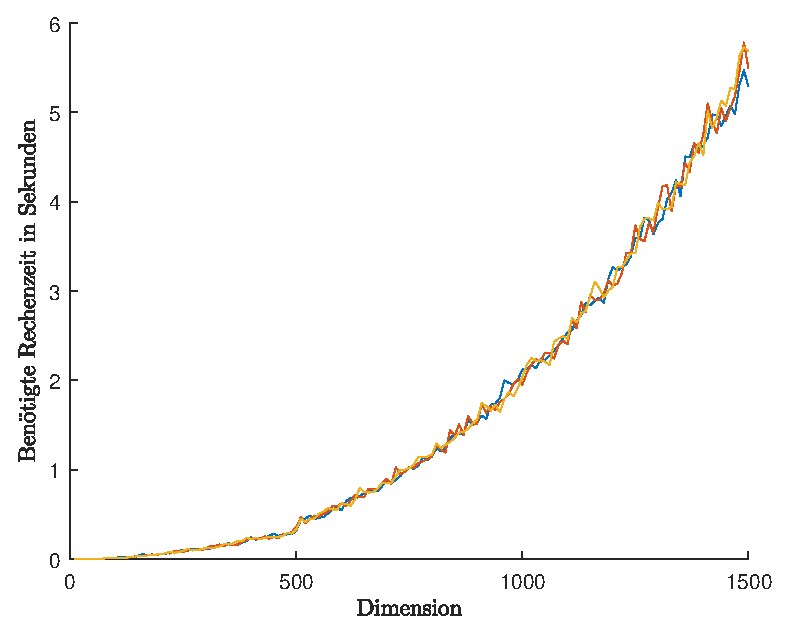
\includegraphics{images/eigLaufzeit}}

\caption{Laufzeitplot bei der Berechnung des Spektrums.}\label{fig:chap5:laufzeit}
\end{figure}

Da das Warten auf Ergebnisse noch h"oherer Dimension etwas Geduld erfordert, zeigt die folgende Tabelle exemplarisch f"unf weitere Rechenresultate. Dabei wurde bei der angegebenen Rechenzeit das arithmetische Mittel bestimmt.

\begin{center}
\begin{tabular}{lccccc}
Dimension & 2000 & 3000 & 4000 & 5000 & 10000 \\
\hline
Rechenzeit in s & $\approx$ 12.2 & $\approx$ 33.3 & $\approx$ 75.6 & $\approx$ 133.1 & $\approx$ 1047.5
\end{tabular}
\end{center}

Die Berechnung best"atigen die theoretisch hergeleitete Laufzeit.
Au"serdem vermitteln diese Werte eine Intuition, von der Gr"o"senordnung von Laufzeiten bei hochdimensionalen Eigenwertproblemen, wie sie etwa bei Berechnungen von Netflix, Facebook oder Amazon vorkommen. Hier sprechen wir von Dimensionen im Millionenbereich.\footnote{Siehe \cite{facebook}, \cite{amazon} und \cite{netflix}.}\\

Die obigen Zahlen motivieren dazu, beim Filtern von Eigenpaaren von einer Berechnung des gesamten Spektrums abzusehen. Wollen wir Eigenpaare durch Ritz-Paare zu einem gegebenen Unterraum ann"ahern, so zeigt sich, dass das Rayleigh-Ritz Verfahren zu einer k"urzeren Laufzeit f"uhrt. Das ist freilich nicht verwunderlich, da das Problem auf eine niedrigere Dimension reduziert wird.\\

Als Hilfsmittel zur Demonstration wurde dieses Mal der Algorithmus \ref{alg:appAlgorithm:rayleighRitz} verwendet. Diese Methode berechnet Ritz-Paare zu einem zuf"allig generierten Suchraum der Dimension $N/5$, wobei $N$ wieder der Dimension von $A$ entspricht. Die Basisvektoren des Suchraumes werden mit der \mcode{orth}-Funktion orthonormiert und die \mcode{eig}-Funktion hilft uns wie zuvor bei der Berechnung von Eigenpaaren. Diesmal jedoch vom Problem der reduzierten Dimension.

\newpage

\begin{figure}[h!]
\centering

\resizebox{.7\textwidth}{!}{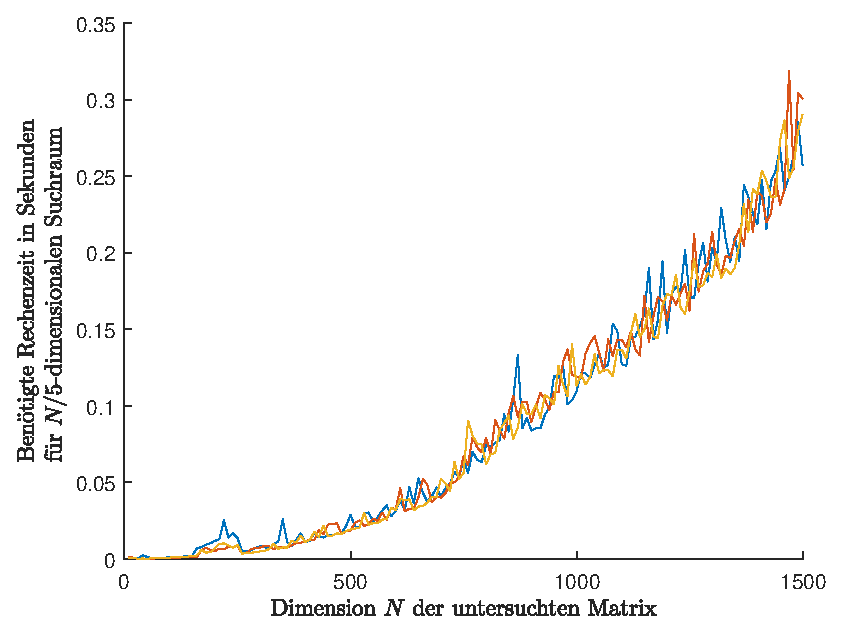
\includegraphics{images/rayleighRitzLaufzeit}}

\caption{Laufzeitplot bei der Berechnung von Ritzpaaren.}\label{fig:chap5:laufzeitRayleighRitz}
\end{figure}

Wenig "uberraschend ist die Laufzeit trotz des Orthonormiervorgangs und zus"atzlicher Matrixmultiplikationen deutlich geringer als zuvor und liegt f"ur die hier betrachteten $N$ unterhalb der Sekundenmarke.\\

Es gibt jedoch die Kehrseite der Medaille: Die Willk"uhrlichkeit bei der Wahl der Suchr"aume spiegelt sich in der G"ute der Ritz-Paare wieder. Um dies einzusehen, w"ahlen wir als G"utekritierum den \emph{minimalen kanonischen Winkel} zwischen dem von den Ritz-Vektoren aufgespannten Unterraum $\mathcal{R}$ und dem von den Eigenvektoren aufgespannten Unterraum $\mathcal{X}$.\\

Diesen minimalen kanonischen Winkel definiert man folgenderma"sen:
\[
\theta_{\min}(\mathcal{R},\mathcal{X}) =
\min
\left\{\arccos\frac{|x^H r|}{\|x\|\|r\|} : r\in\mathcal{R}\setminus\{0\}, x\in\mathcal{X}\setminus\{0\}\right\}.
\]
Sind $R$ und $X$ Matrizen mit $\Bild(R)=\mathcal{R}$ und $\Bild(X)=\mathcal{X}$, so l"asst sich $\theta_{\min}(\mathcal{R},\mathcal{X})$ mit Hilfe der MATLAB-Funktion
\[
\mcode{subspace(R,X)}
\]
n"aherungsweise bestimmen. Dies machen wir uns in Algorithmus \ref{alg:appAlgorithm:ritzVecAngle} zu Nutze.\\

Diese Methode berechnet zun"achst Ritz-Paare bez"uglich eines zuf"allig generierten zweidimensionalen Suchraums. Anschlie"send wird das Minimum aller minimalen kanonischen Winkel zwischen dem von den Ritz-Vektoren aufgespannten Unterraums und allen zweidimensionalen Unterr"aumen, die sich aus Eigenvektoren konstruieren lassen, ermittelt. Die Dimension endet diesmal bei $N=500$, steigert sich aber wie bisher in Zehnerschritten. Erneut wird die Berechnung im Sinne der Konsistenz drei Mal durchgef"uhrt.

\newpage

\begin{figure}[h!]
\centering

\resizebox{.7\textwidth}{!}{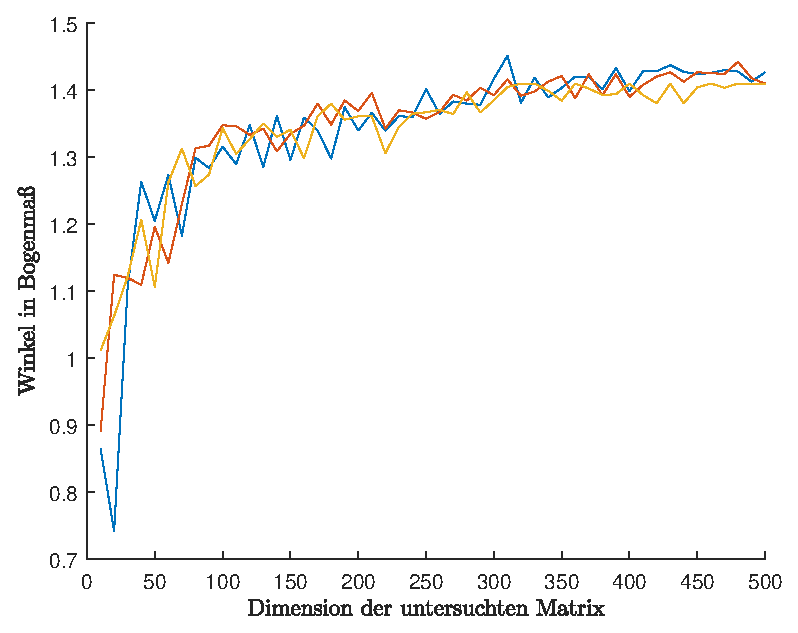
\includegraphics{images/ritzPairAngle}}

\caption{Berechnung des Winkels zwischen Ritz- und Eigenvektoren.}\label{fig:chap5:winkel}
\end{figure}

Nach Konstruktion gilt $\theta_{\min}(\mathcal{R},\mathcal{X})\in[0,\pi/2]$.
Demnach l"asst Abbildung \ref{fig:chap5:winkel} vermuten, dass das nichtiterative Rayleigh-Ritz Verfahren f"ur gewisse Gr"o"senordnungen vollkommen unbrauchbar ist: Mit gr"o"ser werdender Dimension n"ahert sich der Winkel $\pi/2$ an -- die Trefferquote sinkt also.\\

Dem gegen"uber steht die iterative Version des Rayleigh-Ritz Verfahrens: In Algorithmus \ref{alg:appAlgorithm:iterRitzVecAngle} wird getestet, wie sich Ritz-Vektoren und Eigenvektoren im Sinne ihres minimalen kanonischen Winkels ann"ahern. Die Dimension der verglichenen Unterr"aume entsprach dabei erneut 2.
Die Methode zun"achst mit konstant bleibendem Exponenten $k=1$ und im Anschluss mit sich stets um 1 erh"ohendem Exponenten durchgef"uhrt. Im Gegensatz zur Prozedur ohne Iteration ist hier zumindest in dieser kleinen getesteten Stichprobe eine Konvergenz zu erkennen. Dies ist nicht weiter verwunderlich, da die Verwandtschaft zur Potenzmethode dazu f"uhrt, dass der zweidimensionale Suchraum gegen den zweidimensionalen Unterraum konvergiert, welcher von den zwei dominierenden Eigenvektoren aufgespannt wird.

%Viel besser sieht es hingegen mit der iterativen Version des Rayleigh-Ritz Verfahrens aus. Der Algorithmus \ref{alg:appAlgorithm:iterRitzVecAngle} liefert -- ebenfalls f"ur symmetrische Matrizen -- folgenden Plot.\\

\begin{figure}[h!]
\center
\begin{subfigure}[c]{.4\textwidth}
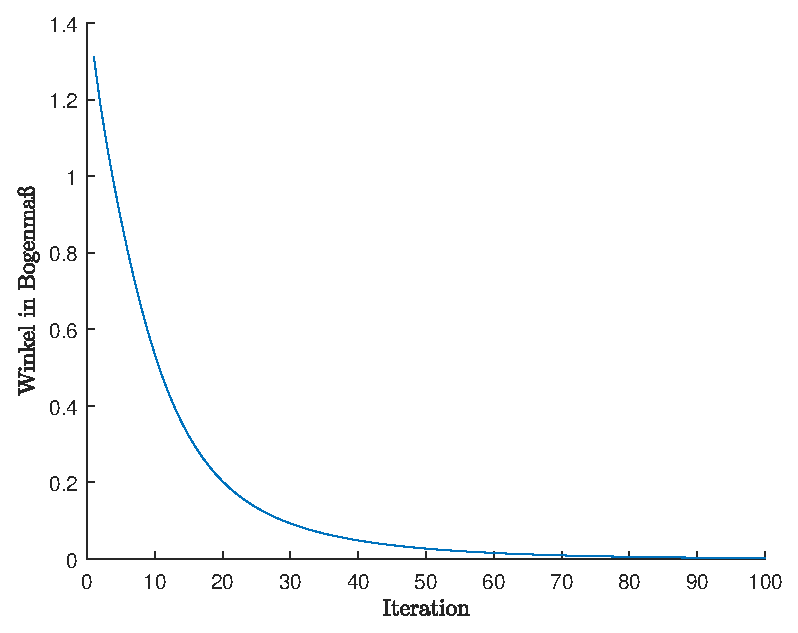
\includegraphics[width=.9\linewidth]{images/iterRRDistConstant}
\subcaption{Konstanter Exponent.}
\end{subfigure}
\begin{subfigure}[c]{.4\textwidth}
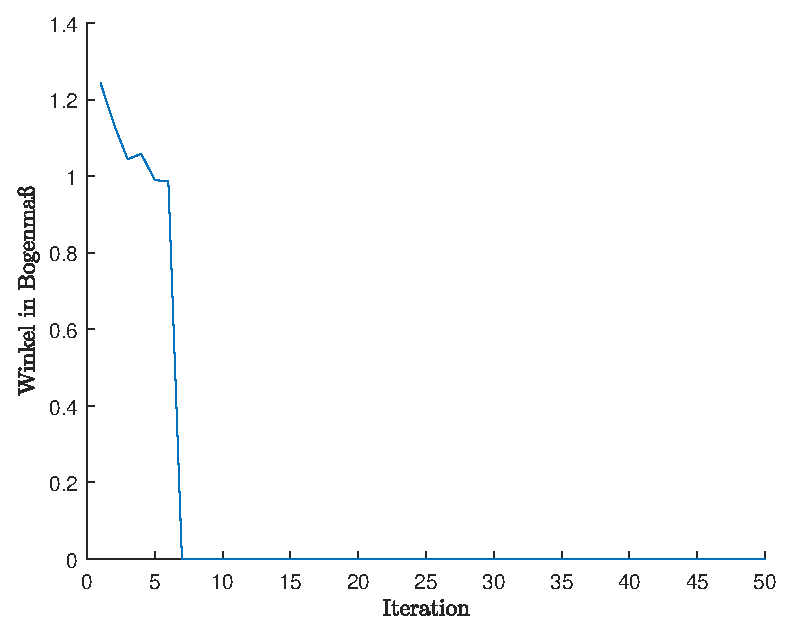
\includegraphics[width=.9\linewidth]{images/iterRRDistIncreasing}
\subcaption{Wachsender Exponent.}
\end{subfigure}
\caption{Unterraumwinkel bei iterativem Rayleigh-Ritz Verfahren.}\label{chap1:im:catinterval}
\end{figure}

\newpage


Zum Abschluss wollen wir unsere Filterkriterien etwas konkreter angeben. Erscheint es bisher so, als h"atte man nicht so recht in der Hand, welche Unterr"aume approximiert werden, wollen wir nun gezielt Teilmengen aus der Menge aller Eigenpaare extrahieren. Dazu betrachten wir abschlie"send den FEAST-Algorithmus.

\section{RKToolbox}

Wir schr"anken uns nun nicht mehr auf das gew"ohnliche Eigenwertproblem ein, sondern betrachten stattdessen allgemeiner das HPD-Eigenwertproblem $(A,B)$ der Dimension $n$. Gesucht sind Eigenpaare, bei denen die Eigenwerte innerhalb eines gegebenen reellen Intervalls $[\lambda_{\min}, \lambda_{\max}]$ liegen sollen.
Zu diesem Zweck wollen wir den FEAST-Algorithmus so implementieren, dass er die gleiche Struktur wie Algorithmus \ref{alg:chap4:beschlRrIteration} hat. Dazu erinnern wir uns an den Fakt, dass das Ersetzen von $\p(B^{-1}A)$ durch eine geeignete rationale Funktion gerade zum FEAST-Algorithmus f"uhrt.\\

Zur Konstruktion dieser Funktion bedienen wir uns an der von G"uttel und Berfjala entwickelten RKToolbox \cite{rkt}. Diese erm"oglicht uns das Erstellen eines sogenannten \mcode{rkfun}-Objektes, mit dessen Hilfe diverse rationale Funktionen konstruiert werden k"onnen. Neben konstanten Funktionen, Tschebyscheff-Polynomen oder Zolotarev'schen N"aherungen an die Wurzelfunktion kann durch den Aufruf
\[
\mcode{r = rkfun('step', k)}
\]
eine rationale Funktion \mcode{r} initialisiert werden, welche die Indikatorfunktion zum Intervall $[-1,1]$ mit einer durch den Parameter $\mcode{k}\in\N$ gesteuerten Genauigkeit approximiert.\footnote{F"ur genauere Ausf"uhrungen wende sich der Leser an die Dokumentation der RKToolbox \cite{rkt}.}\\

Um uns einen Eindruck von einer so initialisierten Funktion zu verschaffen, setzen wir zu Demonstrationszwecken
\[
\mcode{r4 = rkfun('step',4)}\text{,  }\mcode{r5 = rkfun('step',5)}\text{,  }
\mcode{r6 = rkfun('step',6)}
\]
und betrachten den Plot in der Abbildung \ref{fig:chap5:ratFun}. Zun"achst halten wir fest, dass die Indikatorfunktion zumindest nach optischen Kritieren gut approximiert wird. Das ist jedoch kein Zufall.\\

Nach Aussagen G"uttels bedient sich die eben beschriebene Routine bei der Interpolation an Ideen Zolotarevs. Im Wesentlichen werde eine optimale Approximation an die Signums-Funktion auf symmetrischen Intervallen $[-b,-a]$ und $[a,b]$ durch eine M"obiustransformation in eine optimale rationale Approximation der Indikatorfunktion "uberf"uhrt.\footnote{Diese Information entstammt einer m"undlichen R"ucksprache mit G"uttel. Die genaue Konstruktion wird zum Beispiel in \cite[Abschnitt 4]{zol} erkl"art.} Die Abbildung \ref{fig:chap5:ratFun} best"atigt die in \cite[Abschnitt 4]{zol} hergeleiteten Fehlerschranken.

\newpage

\begin{figure}[h!]
\centering

\resizebox{.7\textwidth}{!}{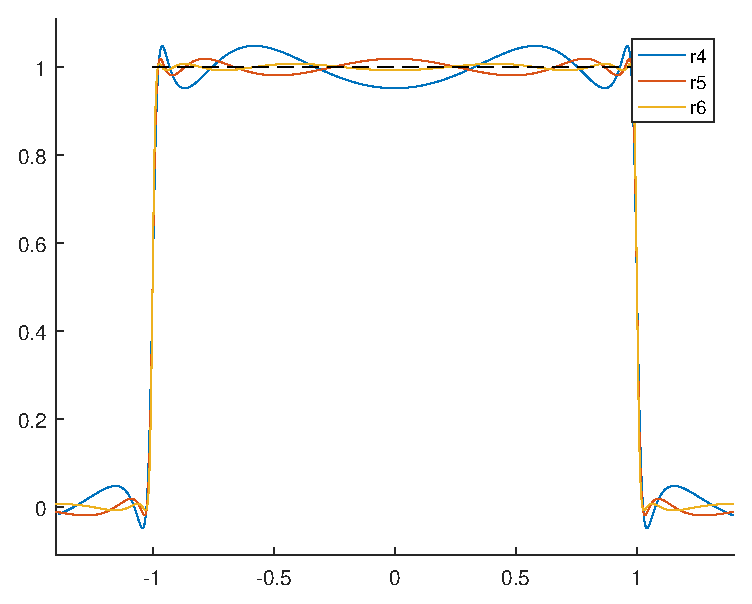
\includegraphics{images/ratFun}}

\caption{Plot der Filterfunktionen \mcode{r4}, \mcode{r5} und \mcode{r6}.}\label{fig:chap5:ratFun}
\end{figure}

Das Einbinden dieser Filterfunktion in die beschleunigte Rayleigh-Ritz Iteration f"uhrt zu der in Algorithmus \ref{alg:appAlgorithm:FEAST} vorgestellten Umsetzung des FEAST-Algorithmus. Hier legen wir zun"achst die Dimension, die Iterationszahl sowie das Intervall, auf dem Eigenwerte bestimmt werden sollen, fest. Da \mcode{rkfun('step',k)} f"ur ein $k\in\N$ standardm"a"sig auf dem Intervall $[-1,1]$ agiert, muss eine entsprechende Transformation auf das gew"unschte Intervall durchgef"uhrt werden.\\

Beispielhaft betrachten wir Eigenwertprobleme $(A,B)$ mit reell symmetrischem $A$ und symmetrisch positiv definitem $B$.
Zu Referenzzwecken bestimmen wir wie bisher mit der MATLAB internen \mcode{eig}-Funktion die Eigenpaare des Eigenwertproblems unter Ber"ucksichtigung des vorgegebenen Intervalls $[1,2.5]$. Zur Approximation der Indikatorfunktion benutzen wir eine \mcode{rkfun('step',5)}-Funktion.\\

Der Algorithmus bestimmt wiederum drei Mal den minimalen kanonischen Winkel zwischen dem durch \mcode{eig} berechneten Eigenraum $\mathcal{X}$ und dem durch FEAST berechneten Eigenraum $\mathcal{R}$. In Abbildung \ref{fig:chap5:feast} zeigt sich, dass bereits im ersten Durchlauf der Winkel zwischen den Unterr"aumen verschwindend gering ist. Damit best"atigt sich die These, dass die beschleunigte Rayleigh-Ritz Iteration in einem Schritt konvergiert, falls $\p(B^{-1}A)$ der Spektralprojektor ist, $m$ der Anzahl der Eigenwerte auf $[1,2.5]$ entspricht und $\p(B^{-1}A)Y_{(0)}$ vollen Rang hat -- denn genau so wurden alle Werte bei der Umsetzung des FEAST-Algorithmus gew"ahlt.\footnote{Vgl. Seite \pageref{eq:quadratur} erster Absatz. F"ur weitere Demonstrationen siehe \cite{feast}.}

\newpage

\begin{figure}[h!]
\centering

\resizebox{.7\textwidth}{!}{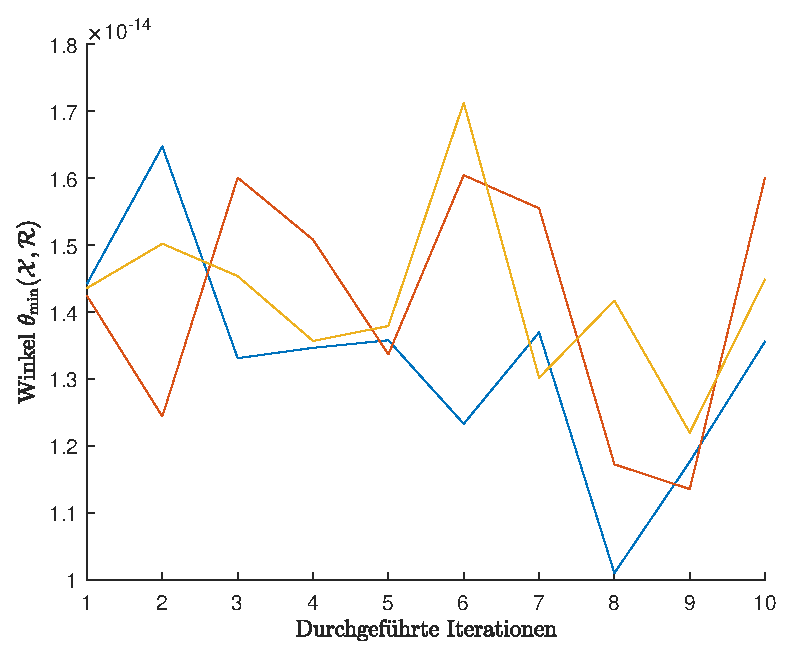
\includegraphics{images/feastAngle}}

\caption{Plot von Algorithmus \ref{alg:appAlgorithm:FEAST}.}\label{fig:chap5:feast}
\end{figure}

Zum Abschluss f"uhren wir einen weiteren Test durch. We verh"alt sich blabla wenn nahe intervallgrenzen?
